\documentclass[a4paper,12pt]{article}

\usepackage{graphicx} % Required for inserting images
\usepackage{amsmath,amssymb,amsfonts}
\usepackage{subcaption}
\usepackage{geometry}
\usepackage{times}
\usepackage{graphicx}
\usepackage{float}
\usepackage{listings}
\usepackage{xcolor}
\usepackage{multirow}
\usepackage{titlesec} % To customize section font size
\usepackage{pdfpages} % Include PDF files

% Set page margins
\geometry{a4paper, top=1in, bottom=0.8in, left=1.1in, right=0.8in}

% Add page numbering
\pagestyle{plain}

% Set no paragraph indent
\setlength{\parindent}{0pt}

% -----------------------
% Section Font Customization
% -----------------------

\titleformat{\section}
{\normalfont\fontsize{14}{16}\bfseries}{\thesection}{1em}{}

\titleformat{\subsection}
{\normalfont\fontsize{14}{16}\bfseries}{\thesubsection}{1em}{}



\begin{document}
	\section{Experiment No. 4}
	
	\section{Experiment Title }
	Observation of the External Characteristic Curve of Synchronous Generator for different type of
	Load.
	
	\section{Objective}
	
	The objectives of this lab are as follows:
	\begin{itemize}
		\item TTo Observe the generator’s characteristic curve (terminal voltage vs. load current) under
		different type of load: Resistive(R), Inductive(L), Capacitive(C).
		\item To analyze how resistive, inductive, and capacitive loads affect a synchronous generator’s
		performance .
		
		
	\end{itemize}
	
	\section{Theory}
	

A synchronous generator (alternator) converts mechanical energy into electrical energy by electromagnetic induction. It operates on the principle that a rotating magnetic field induces an electromotive force (EMF) in the stationary armature windings according to Faraday's Law.

The terminal voltage \( V_t \) of a synchronous generator depends on the load current \( I_L \), the nature of the load (resistive, inductive, or capacitive), and the internal parameters of the machine. The external characteristic of a synchronous generator is the graph plotted between terminal voltage \( V_t \) and load current \( I_L \) at a constant speed and excitation.

\subsection{Voltage Equation and Phasor Representation}

The internal generated voltage \( E_a \) is related to the terminal voltage \( V_t \) by the following phasor equation:

\[
E_a = V_t + I_a(R_a + jX_s)
\]

Where:
\begin{enumerate}
	\item \( E_a \) = Internal EMF (V)
	\item \( V_t \) = Terminal voltage (V)
	\item \( I_a \) = Armature current (A)
	\item \( R_a \) = Armature resistance ($\Omega$)
	\item \( X_s \) = Synchronous reactance ($\Omega$)
\end{enumerate}

This phasor relationship illustrates how resistive and reactive voltage drops contribute to the total voltage required to supply a given load.

\subsection{Load Types and Their Effects on Terminal Voltage}

\subsubsection*{Resistive Load (R)}

	 Voltage and current are in phase (\( \phi = 0^\circ \)).
	 Terminal voltage decreases linearly and moderately with increasing load current.
	 Voltage drop is mainly due to \( I_aR_a \) and a smaller component of \( I_aX_s \).
\begin{figure}[H]
	\centering
	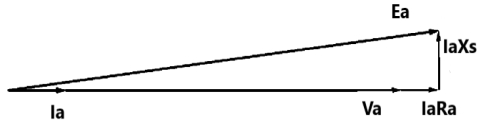
\includegraphics[width=0.7\linewidth]{Images/2}
	\caption{ Phase Diagram for Resistive Load}
	\label{fig:2}
\end{figure}
	 Armature reaction is minimal as the power factor is unity.


\subsubsection*{Inductive Load (L)}

	 Current lags behind voltage (\( \phi > 0^\circ \)).
	 Terminal voltage drops significantly as load increases.
	 The lagging current causes a demagnetizing armature reaction, reducing the effective main field.
	 \begin{figure}[H]
	 	\centering
	 	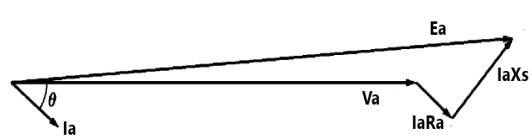
\includegraphics[width=0.7\linewidth]{Images/3}
	 	\caption{Phase Diagram for Inductive Load}
	 	\label{fig:2}
	 \end{figure}
	 Voltage drop is due to both \( I_aX_s \) and the weakened magnetic field.


\subsubsection*{Capacitive Load (C)}

	 Current leads voltage (\( \phi < 0^\circ \)).
	 Terminal voltage tends to increase with increasing load current.
	 The leading current produces a magnetizing armature reaction, strengthening the main field.
	 
	\begin{figure}[H]
		\centering
		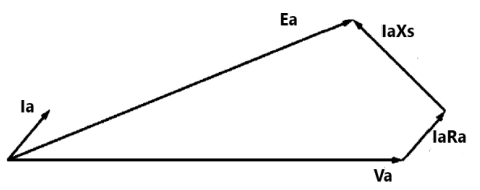
\includegraphics[width=0.7\linewidth]{Images/4}
		\caption{  Phase Diagram for Capacitive Load}
		\label{fig:2}
	\end{figure}
	
	This results in a rise in terminal voltage, especially at higher loads.




The external characteristics of a synchronous generator under different load conditions can be summarized as:
\begin{enumerate}
	\item \textbf{Lagging Power Factor (Inductive Load)}: Sharp downward curve of \( V_t \) with increasing \( I_a \).
	\item \textbf{Unity Power Factor (Resistive Load)}: Moderate and nearly linear decrease in \( V_t \).
	\item \textbf{Leading Power Factor (Capacitive Load)}: Slight increase in \( V_t \) with increasing \( I_a \).
\end{enumerate}

Understanding these characteristics is vital for the stable operation and efficient control of synchronous generators in power systems.

\subsection{Voltage Regulation}

The voltage regulation of the generator can be calculated using the formula:

\[
\text{Voltage Regulation (\%)} = \frac{E_f - V_t}{V_t} \times 100
\]

Where \( E_f \) is the no-load EMF and \( V_t \) is the full-load terminal voltage.


	
	\newpage
	\section{Circuit Diagram}
	\begin{figure}[H]
		\centering
		
			\centering
			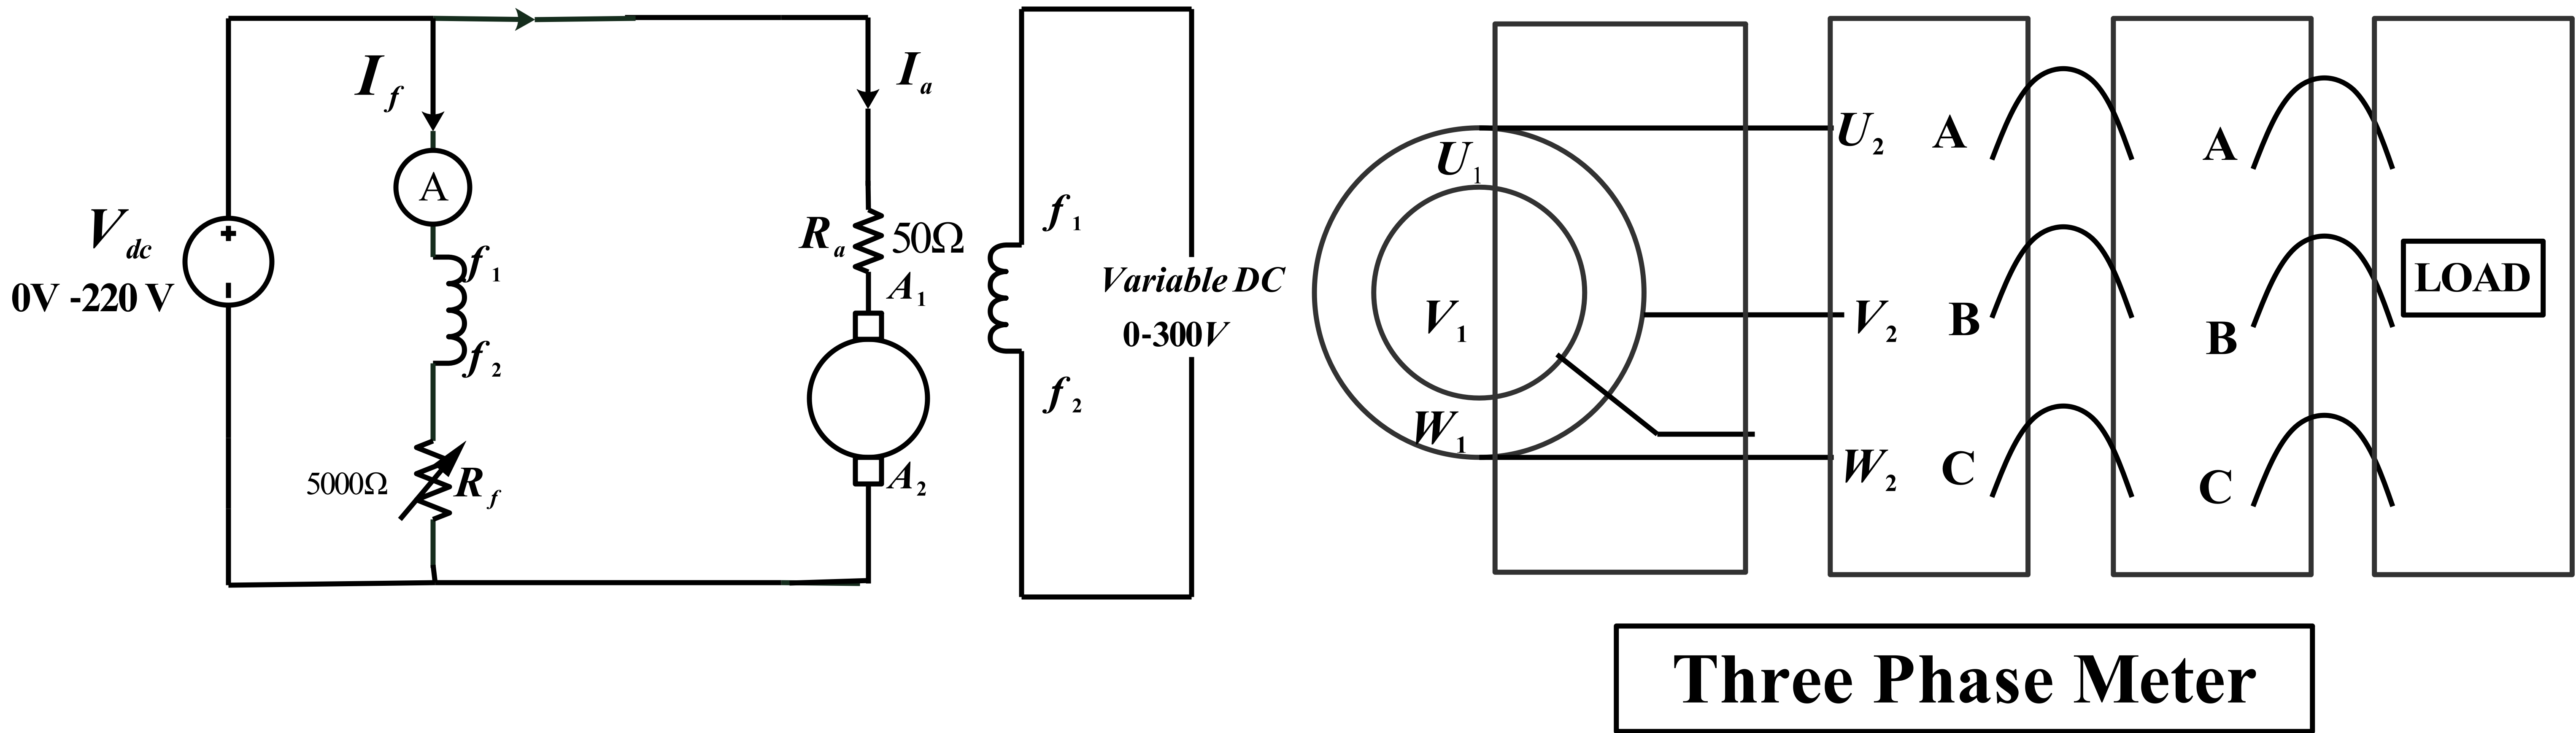
\includegraphics[width=1\textwidth]{Images/6}
			\caption{Circuit Diagram of Open Circuit Test.}
			
	
		
	\end{figure}
	
	\section{Required Apparatus}
	\begin{enumerate}
		\item \textbf{DC Motor}
		\begin{enumerate}
			\item Power: 300W , Speed: 3000 rpm
			\item Voltage: 220V
			\item \textbf{Excitation (Series)}: D1-D2, Current: 1.9A, \textbf{Excitation (Separate)}: F1-F2, Current: 1.8A, Excitation Voltage: 220V, Excitation Current: 0.1A
			
		\end{enumerate}
		
		\item \textbf{Synchronous Generator}
		\begin{enumerate}
			\item Power: 350W ,Power Factor: $\cos\phi = 1$ ,Speed: 3000 rpm
			
			\item Voltage: 400V (star) / 230V (delta) ,Current: 0.7A (star) / 1.2A (delta) 
			\item Excitation Voltage: 220V ,Excitation Current: 0.45A
			
		\end{enumerate}
		
		\item \textbf{Resistors}
		\begin{enumerate}
			\item 50$\Omega$: Power = 500W, Current = 3.16A
			\item 200$\Omega$: Power = 500W, Current = 1.58A
			\item 5000$\Omega$: Power = 500W, Current = 0.31A
		\end{enumerate}
		
		\item \textbf{Tachometer}
		\begin{enumerate}
			\item For 0.6V/rev: 300V at 5000 RPM , For 2mV/rev: 10V at 5000 RPM
			\item Maximum Current: 0.07A
			\item Maximum Speed: 5000 RPM
		\end{enumerate}
		
		\item \textbf{AC Multimeter}
		\begin{enumerate}
			\item 500V AC RMS
			\item 5A
		\end{enumerate}
	\end{enumerate}
	
	
	
	
	\newpage
	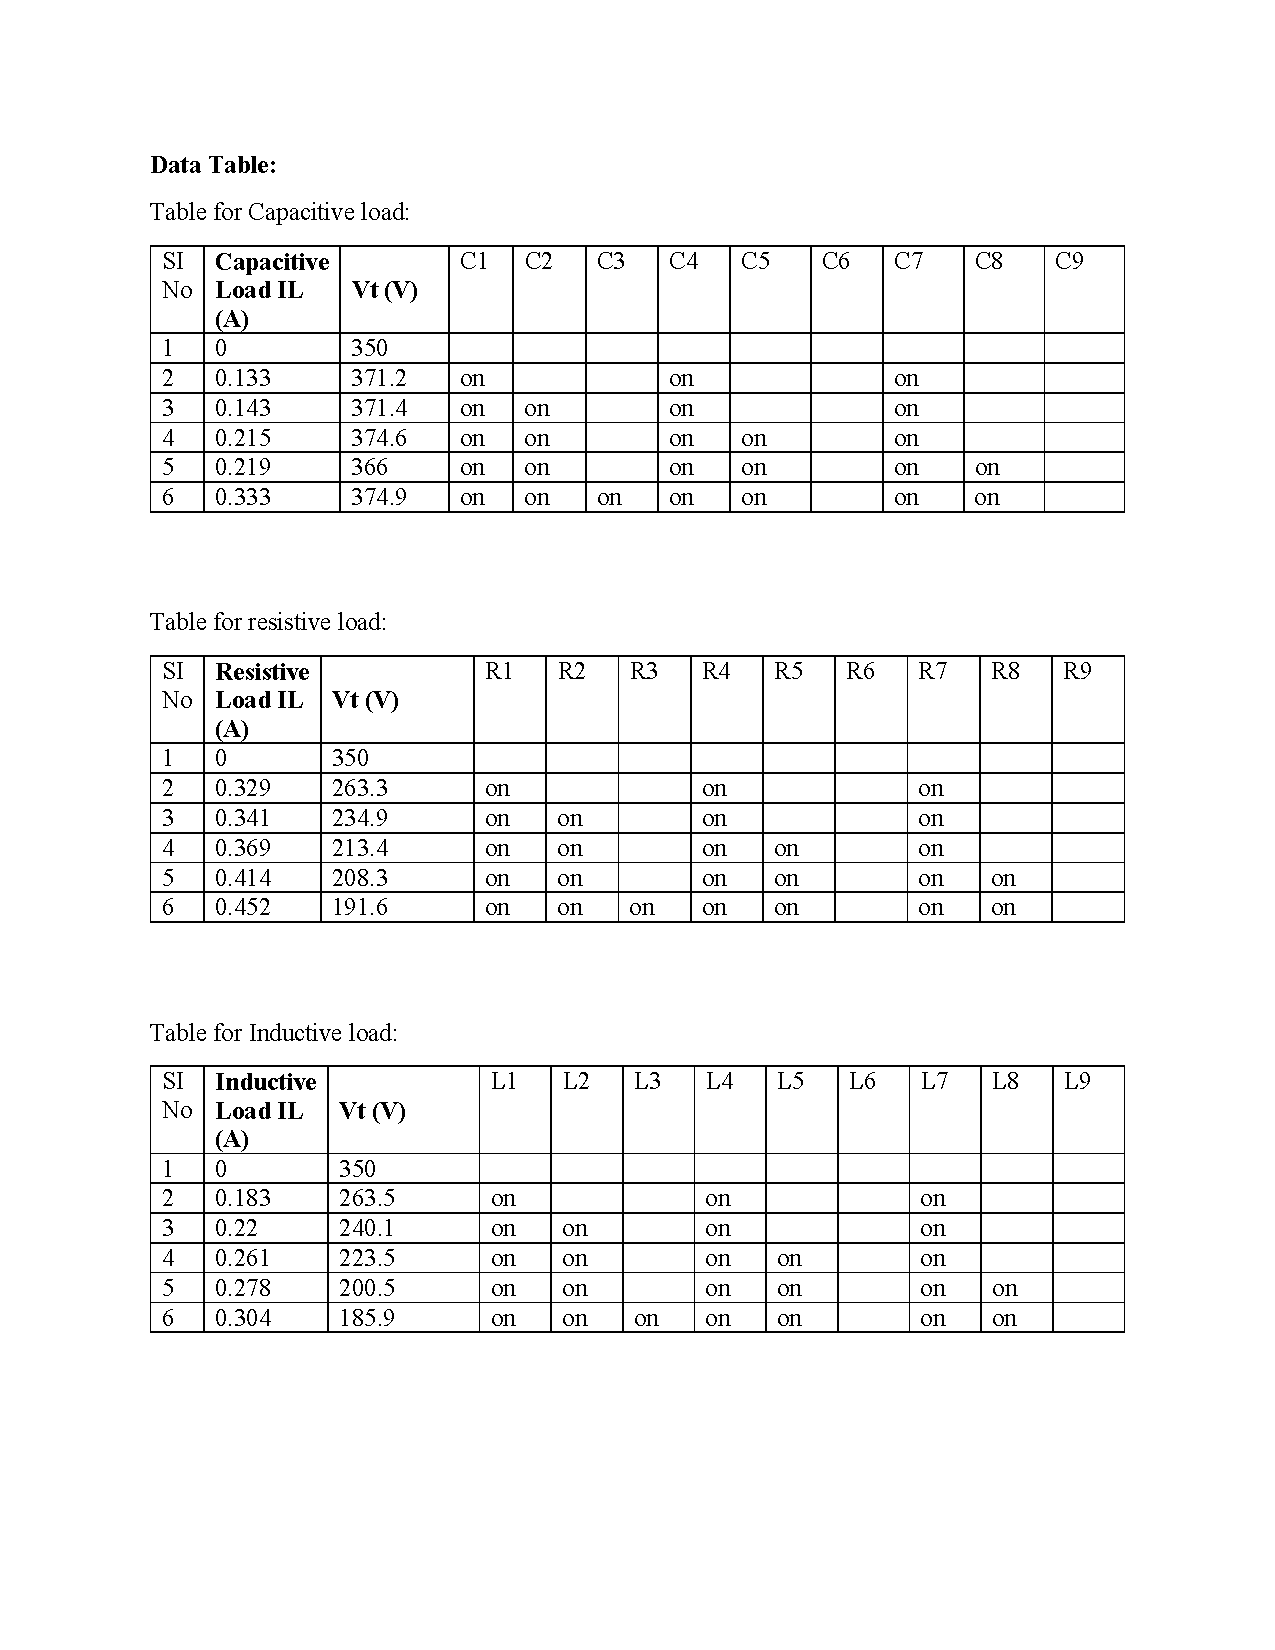
\includepdf[pages=-, fitpaper=true]{datatable.pdf}
	
	
	
	\section{Graph}
	\begin{figure}[H]
		\centering
		
			\centering
			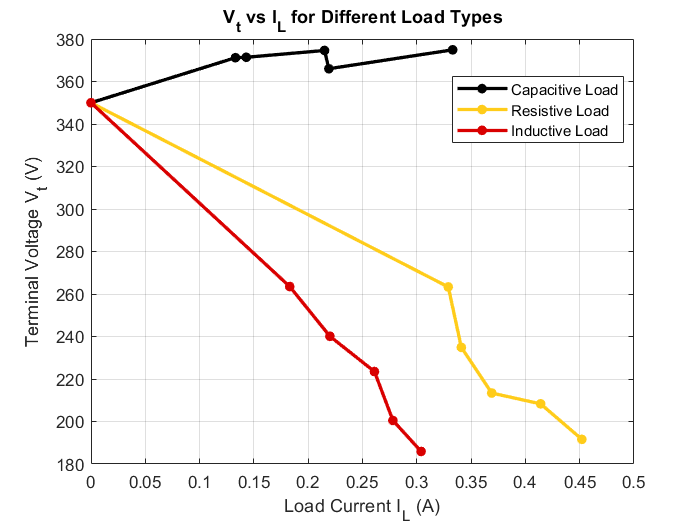
\includegraphics[width=.94\linewidth]{Images/1}
			\caption{$V_{t}$ vs $I_L$ Graph }
			
	
		
	
	\end{figure}
	
	\section{Discussion}
	
	

In theexperiment ,the external characteristics of the synchronous generator were observed by varying the load type and measuring the terminal voltage \( V_t \) against the load current \( I_L \). Three types of loads—capacitive, resistive, and inductive—were applied separately, and their effects on terminal voltage were recorded.

Under capacitive loading, it was observed that the terminal voltage increased slightly with the increase in load current. This was due to the leading power factor, where the armature reaction had a magnetizing effect, strengthening the main field. As a result, the voltage rise was seen, especially at higher currents.

When a resistive load was applied, the terminal voltage decreased nearly linearly as the load current increased. This behavior was expected due to the in-phase nature of current and voltage (\( \phi = 0^\circ \)), and the voltage drop was mainly caused by the armature resistance \( I_aR_a \) and a small component of \( I_aX_s \).

In terms of inductive load, a sharp decline in terminal voltage was recorded as the load current increased. The lagging current created a demagnetizing armature reaction, which weakened the main field, leading to a significant drop in \( V_t \). This effect was intensified by the presence of synchronous reactance \( X_s \), which increased the voltage drop across the internal impedance.

Overall, the experimental results were consistent with the theoretical expectations for each load type.

	
\end{document}